%%
%% cap3.tex
%% 
%% Made by Carlos Calcaneo Roldan
%% Login   <calcaneo@jogrant>
%% 
%% Started on  Mon Jul 22 15:03:25 2019 Carlos Calcaneo Roldan
%% Last update Time-stamp: <2020-jul-29.miércoles 19:05:05 ()>
%%

\chapter{Halos de Materia Oscura}
\setcounter{equation}{0}

Con la intención de conocer y diferenciar las diferentes cosmologías, en nuestro estudio de los halos de materia oscura, optamos por realizar fue una variedad de simulaciones de materia oscura. Desde simulaciones con cosmologías de Universos planos ($\Omega = 1$), asi como cosmologías  de universos con densidades sub-criticas ($\Omega < 1$) y super-criticas ($\Omega > 1$).

%%%%%%%%EL TExto Comienza abajo de aquí! 
 \section{Universo con cosmología  \texorpdfstring{$\Omega_\lambda = 0.691$, $\Omega_0 = 0.309$ }{Omega lambda = 0.691, Omega 0 = 0.309}  }


En la evolución del Universo, la materia del Universo se comenzó a agrupar lentamente en lo que llamamos halos. En un principio la materia parece una nube difusa sin estructuras internas, después de un tiempo en el que se esta agrumando, pequeñas estructuras de materia se empiezan a formar. Las primeras estructuras son pocas como se aprecia en la figura \ref{fig:EvoNumTotHalos}. Las estructuras tardan tiempo en aparecer y eventualmente hay un aumento acelerado en la cantidad halos que se forman y mas hacia al presente vemos un pico donde empiezan a disminuir el total de halos.

\begin{figure}
    \centering
    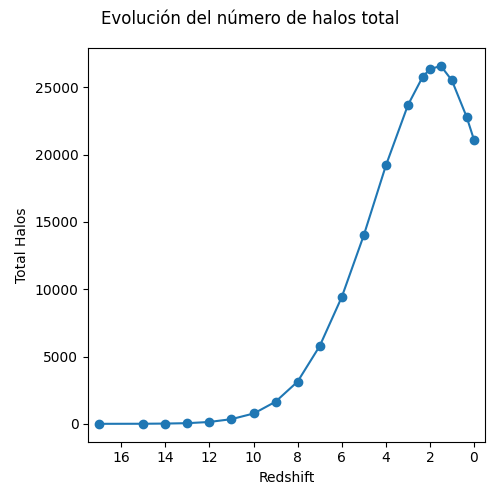
\includegraphics[scale = 0.65]{TotalHalos.png}
    \caption[Evolución del número de halos en un Universo $\Omega_\lambda = 0.691 $, $\Omega_0 = 0.309$]{\small Se muestra el numero de halos y como cambia la cantidad conforme evoluciona el Universo en una cosmología $\Omega_\lambda = 0.691 $ y $\Omega_0 = 0.309$.}
    \label{fig:EvoNumTotHalos}
\end{figure}

En la figura \ref{fig:MassDistCanonRunSep} y \ref{fig:MassDistCanonRun} podemos observar que aunque disminuyen la cantidad de halos después del redshift 2, podemos ver que comienzan a aparecer estructuras mas masivas. Las estructuras en un principio son pequeñas y escasas y conforme el el Universo evoluciona podemos ver una gran cantidad de halos pequeños a medianos. Mas al presente, se observan que las estructuras son cada vez mas grandes, aunque no en gran cantidad.

\begin{figure}
    \centering
    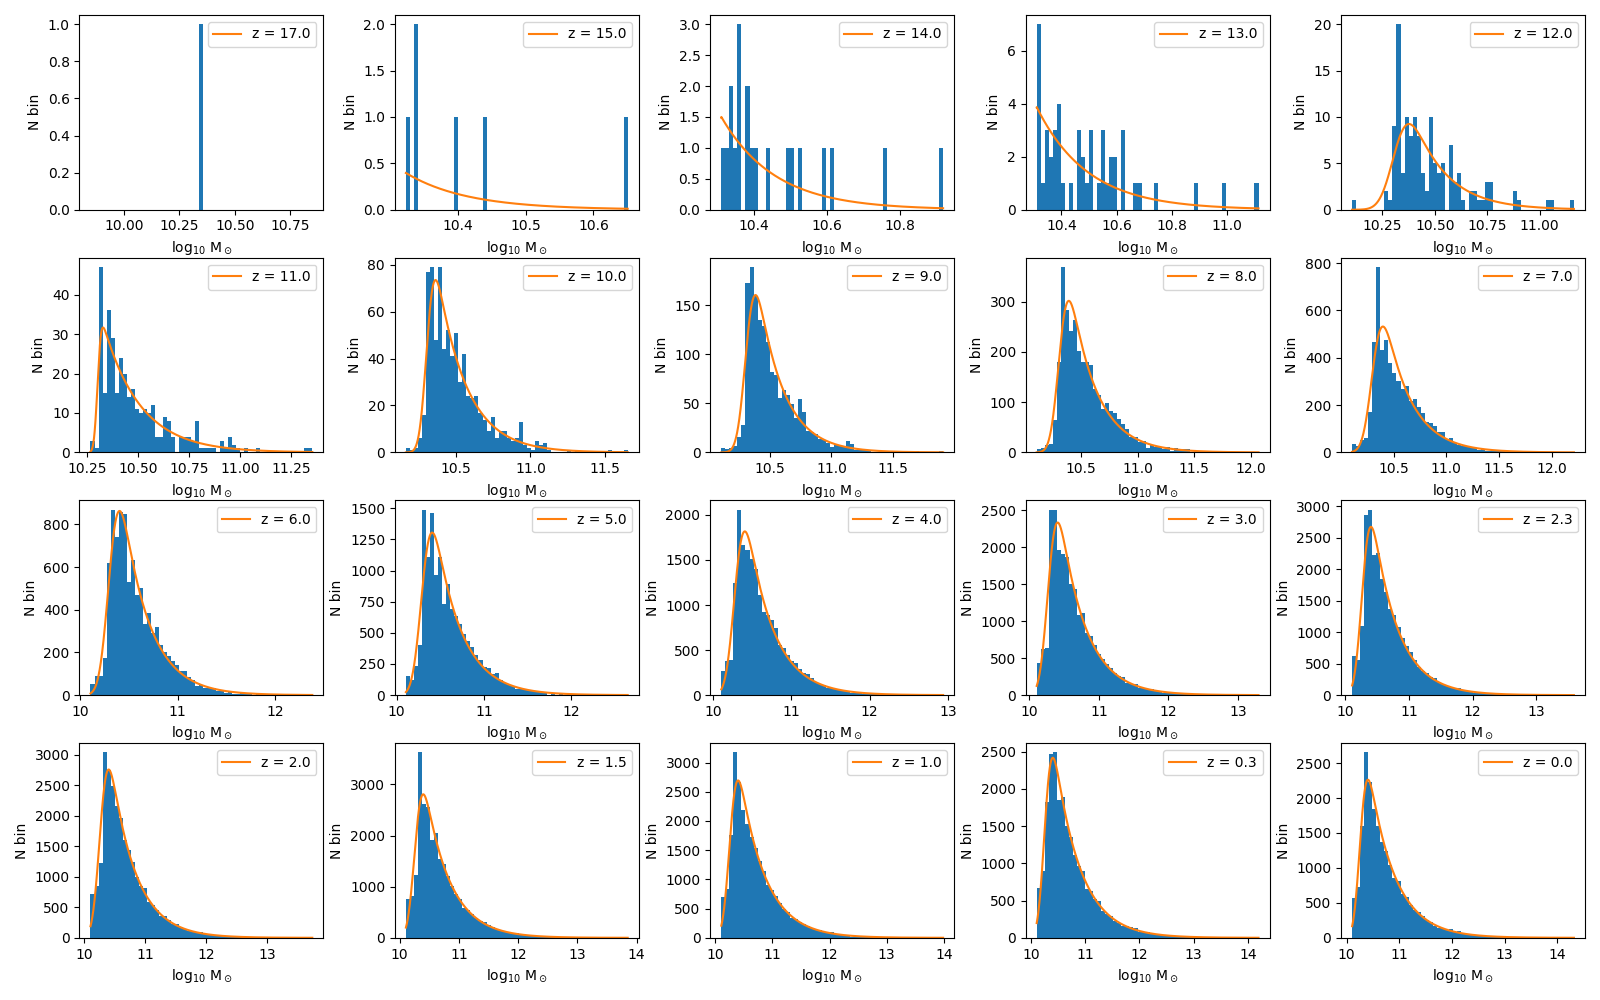
\includegraphics[width = 1\linewidth]{MassDistCanonRunSep.png}
    \caption[Distribución de masa en la evolución de un Universo $\Omega_\lambda = 0.691 $, $\Omega_0 = 0.309$]{\small Se muestra la distribución de la masa conforme evoluciona el Universo en una cosmología $\Omega_\lambda = 0.691 $ y $\Omega_0 = 0.309$. Se observa como aumentan la cantidad de halos cada vez mas masivos.}
    \label{fig:MassDistCanonRunSep}
\end{figure}

\begin{figure}
    \centering
    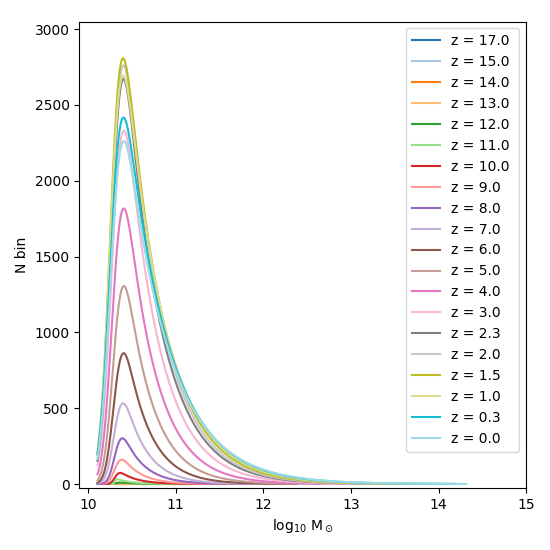
\includegraphics[scale=0.65]{MassDistCanonRun.png}
    \caption[Comparación de distribución de masa Universo $\Omega_\lambda = 0.691 $, $\Omega_0 = 0.309$]{\small Comparación de las distribuciones de masa durante la evolución del Universo $\Omega_\lambda = 0.691 $, $\Omega_0 = 0.309$. Se observa como crece la cantidad de halos de materia oscura, asi como el tamaño de estos.}
    \label{fig:MassDistCanonRun}
\end{figure}

% En las figuras \ref{fig:MassDistCanonRun}\ref{fig:MassStatsCanonRun} podemos apreciar como el tiempo, los halos de materia oscura comienzan a ser mas masivos. También vemos que la variedad 

\begin{figure}
    \centering
    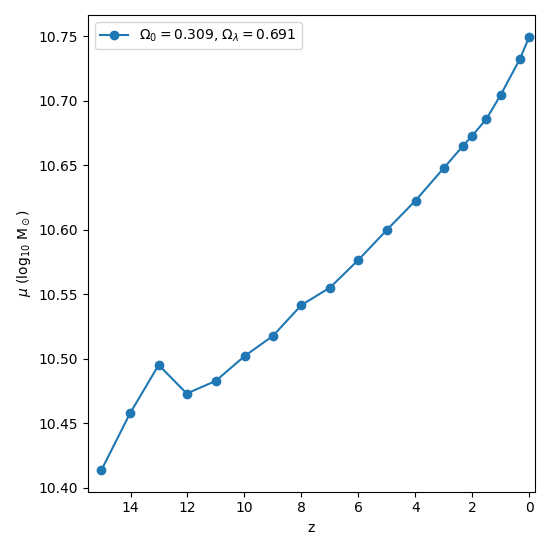
\includegraphics[width = 0.49\linewidth]{RunCanonMassMean.png}
    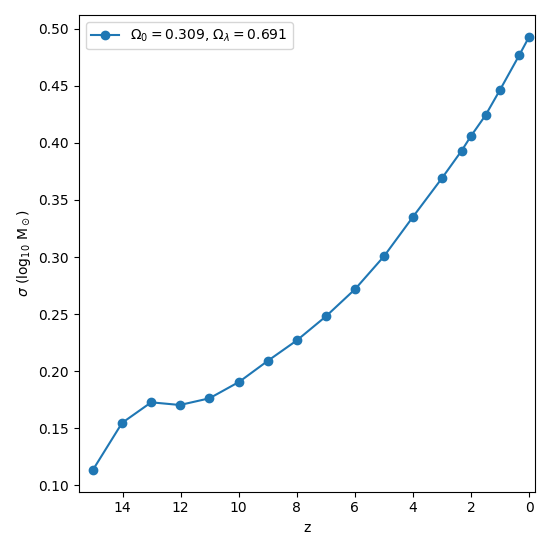
\includegraphics[width = 0.49\linewidth]{RunCanonMassStd.png}
    \caption[Media y desviación estándar de la distribución de masa de un Universo $\Omega_\lambda = 0.691 $, $\Omega_0 = 0.309$]{\small En la izquierda se muestra la masa media de los halos de materia oscura y se observa como cambia durante la evolución del Universo. En la derecha se muestra la desviación estándar de la masa, la cual nos muestra la variedad que hay de los halos de materia oscura.}
    \label{fig:MassStatsCanonRun}
\end{figure}

\begin{figure}
    \centering
    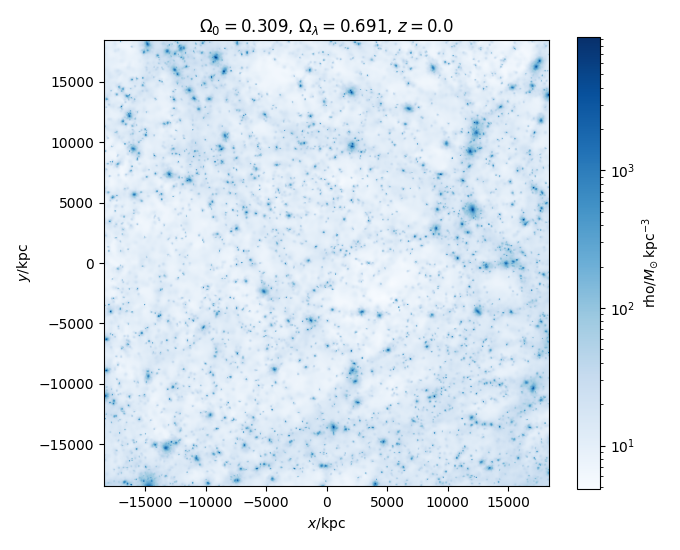
\includegraphics[width = 0.65\linewidth]{RunCanonZ0Rho.png}
    \caption[Mapa de densidad de un Universo $\Omega_\lambda = 0.691 $, $\Omega_0 = 0.309$ en z=0]{\small Mapa de densidad de la simulación en redshift 0 de una cosmología $\Omega_\lambda = 0.691 $, $\Omega_0 = 0.309$.}
    \label{fig:CanonRunDensityMap}
\end{figure}





\section{Cúmulo proyectado sobre el plano de S2}


